\documentclass[twoside]{article}

\usepackage{aistats2022}

\usepackage[round]{natbib}
\renewcommand{\bibname}{References}
\renewcommand{\bibsection}{\subsubsection*{\bibname}}

% If you use BibTeX in apalike style, activate the following line:
\bibliographystyle{apalike}


\usepackage{xr}
\usepackage{amssymb,amsmath,amsthm}
\newtheorem{theorem}{Theorem}
\theoremstyle{definition}
\newtheorem{definition}[theorem]{Definition}
\newtheorem{assumption}[theorem]{Assumption}
\newtheorem{proposition}[theorem]{Proposition}
\newtheorem{lemma}[theorem]{Lemma}
\newtheorem{claim}[theorem]{Claim}
\newtheorem{example}[theorem]{Example}
\newtheorem{corollary}[theorem]{Corollary}
\theoremstyle{remark}
\newtheorem{remark}[theorem]{Remark}
\usepackage[bold]{hhtensor}

\usepackage{hyperref}
\usepackage{cleveref}
\usepackage{mathtools}
\usepackage{booktabs}
\usepackage{float}
\usepackage{braket}
\usepackage{dsfont}
\usepackage{graphbox}
\usepackage{pgf}
\usepackage{comment}
\usepackage{subcaption}
\usepackage{enumitem}

\crefname{assumption}{assumption}{assumptions}
\Crefname{assumption}{Assumption}{Assumptions}
\crefname{proposition}{proposition}{propositions}
\Crefname{proposition}{Proposition}{Propositions}
\crefname{lemma}{lemma}{lemmas}
\Crefname{lemma}{Lemma}{Lemmas}
\crefname{remark}{remark}{remarks}
\Crefname{remark}{Remark}{Remarks}

\DeclarePairedDelimiterX{\infdivx}[2]{(}{)}{%
  #1\;\delimsize\|\;#2%
}
\newcommand{\infdiv}{D\infdivx}

\DeclareMathOperator*{\cov}{cov}

\newcommand{\dd}{\mathrm{d}}

\newcommand{\cE}{\mathcal{E}}
\newcommand{\cL}{\mathcal{L}}
\newcommand{\cO}{\mathcal{O}}
\newcommand{\cP}{\mathcal{P}}
\newcommand{\cQ}{\mathcal{Q}}
\newcommand{\cS}{\mathcal{S}}

\newcommand{\eps}{\varepsilon}
\newcommand{\pd}{\partial}

\newcommand{\dist}{\mathrm{dist}}
\newcommand{\simiid}{\overset{\text{iid}}{\sim}}

\newcommand{\vb}{\vec{b}}
\newcommand{\vv}{\vec{v}}
\newcommand{\vx}{\vec{x}}
\newcommand{\vy}{\vec{y}}
\newcommand{\veta}{\vec{\eta}}

\newcommand{\mI}{\matr{I}}
\newcommand{\mM}{\matr{M}}

\newcommand{\RR}{\mathbb{R}}
\newcommand{\EE}{\mathbb{E}}
\newcommand{\PP}{\mathbb{P}}

\newcommand{\cN}{\mathcal{N}}

\newcommand{\feynman}[1]{{\color{blue}{(Feynman: {#1})}}}
\newcommand{\liam}[1]{{\color{green}{(Liam: {#1})}}}
\newcommand{\michael}[1]{{\color{purple}{(Michael: {#1})}}}


\makeatletter
\newcommand*{\addFileDependency}[1]{% argument=file name and extension
  \typeout{(#1)}
  \@addtofilelist{#1}
  \IfFileExists{#1}{}{\typeout{No file #1.}}
}
\makeatother

\newcommand*{\myexternaldocument}[1]{%
    \externaldocument{#1}%
    \addFileDependency{#1.tex}%
    \addFileDependency{#1.aux}%
}

\myexternaldocument{ftvi_aistats}

% If your paper is accepted, change the options for the package
% aistats2022 as follows:
%
%\usepackage[accepted]{aistats2022}
%
% This option will print headings for the title of your paper and
% headings for the authors names, plus a copyright note at the end of
% the first column of the first page.

% If you set papersize explicitly, activate the following three lines:
%\special{papersize = 8.5in, 11in}
%\setlength{\pdfpageheight}{11in}
%\setlength{\pdfpagewidth}{8.5in}

% If you use natbib package, activate the following three lines:
%\usepackage[round]{natbib}
%\renewcommand{\bibname}{References}
%\renewcommand{\bibsection}{\subsubsection*{\bibname}}

% If you use BibTeX in apalike style, activate the following line:
%\bibliographystyle{apalike}

\begin{document}

% If your paper is accepted and the title of your paper is very long,
% the style will print as headings an error message. Use the following
% command to supply a shorter title of your paper so that it can be
% used as headings.
%
%\runningtitle{I use this title instead because the last one was very long}

% If your paper is accepted and the number of authors is large, the
% style will print as headings an error message. Use the following
% command to supply a shorter version of the authors names so that
% they can be used as headings (for example, use only the surnames)
%
%\runningauthor{Surname 1, Surname 2, Surname 3, ...., Surname n}

% Supplementary material: To improve readability, you must use a single-column format for the supplementary material.
\onecolumn
\aistatstitle{
Supplementary Material for ``Fat--Tailed Variational Inference with Anisotropic Tail Adaptive Flows''}

\section{Proofs}
\label{sec:proofs}

\begin{proof}[Proof of \Cref{thm:distn_class_closed}]
  \label{proof:distn_class_closed}
  Let $X$ be a random variable from either $\cE_\alpha^p$
  or $\cL_\alpha^p$.
  Its concentration function
  \cite[Equation 1.6]{ledoux2001concentration}
  is given by
  \[
    \alpha_X(r)
    \coloneqq \sup \{ \mu\{x : d(x,A) \geq r\}; A \subset \text{supp}~X, \mu(A) \geq 1/2\}
    = \PP(\lvert X - m_X \rvert \geq r)
  \]
  Under Assumption 1, $f_\theta$ is Lipschitz (say with Lipschitz
  constant $L$) so by \cite[Proposition 1.3]{ledoux2001concentration},
  \[
    \PP(\lvert f_\theta(X) - m_{f_\theta(X)}\rvert \geq r)
    \leq 2 \alpha_X(r/L)
    = \cO(\alpha_X(r/L)),
  \]
  where $m_{f_\theta(X)}$ is a median of $f_\theta(X)$.
  Furthermore, by the triangle inequality
  \begin{align}
    \PP(\lvert f_\theta(X) \rvert \geq r)
    &= \PP(\lvert f_\theta(X) - m_{f_\theta(X)} + m_{f_\theta(X)} \rvert \geq r) \nonumber\\
    &\leq \PP(\lvert f_\theta(X) - m_{f_\theta(X)}\rvert \geq r - \lvert m_{f_\theta(X)}\rvert ) \nonumber\\
    &= \cO(\PP(\lvert f_\theta(X) - m_{f_\theta(X)}\rvert \geq r)) \nonumber\\
    &= \cO(\alpha_X(r/L)) \label{eq:pushforward-conc-fn}
  \end{align}
  where the asymptotic equivalence holds because $\lvert m_{f_\theta(X)} \rvert$ is independent of $r$.
  When $X \in \cE_\alpha^p$, \Cref{eq:pushforward-conc-fn} implies
  \[
    \PP(\lvert f_\theta(X) \rvert \geq r)
    = \cO(e^{-\frac{\alpha}{L} r^p}) \implies f_\theta(X) \in \overline{\cE}_{\alpha/L}^p,
  \]
  from whence we find that the Lipschitz transform of exponential-type
  tails continues to possess exponential-type tails with the same
  class index $p$, although the tail parameter may have changed. Hence,
  $\overline{\cE^p}$ is closed under Lipschitz maps for each $p \in \RR_{>0}$.
  On the other hand, when $X \in \cL_\alpha^p$, \Cref{eq:pushforward-conc-fn} also implies that
  \begin{align*}
    \PP(\lvert f_\theta(X) \rvert \geq r)
    &= \cO(e^{-\alpha (\log (r/L))^p})
    % &= \cO(e^{-\alpha (\log r)^p} e^{-\alpha (-\log L)^p}) \\
    = \cO(e^{-\alpha (\log r)^p}),
  \end{align*}
  and therefore, $f_\theta(X) \in \overline{\cL_\alpha^p}$.
  Unlike exponential-type tails, Lipschitz transforms of
  logarithmic-type tails not only remain logarithmic, but
  their tails decay no slower than a logarithmic-type tail
  of the same class index with the \emph{same} tail parameter $\alpha$.
  This upper bound suffices to show closure under Lipschitz maps for the
  ascending family $\overline{\cL_\alpha^p}$.
\end{proof}

\begin{proof}[Proof of \Cref{corr:heavy_to_light}]
    Let $f_\theta$ be as before with the additional assumptions.
    Since $f_\theta$ is a smooth continuous bijection, it is a diffeomorphism.
    Furthermore, by assumption $f_\theta$ has invertible Jacobian on the closure of its
    domain hence $\sup_{x \in \text{dom}~f_\theta} \lvert (f_\theta)'(x) \rvert \geq M > 0$.
    By the inverse function theorem, $(f_\theta)^{-1}$ exists and is
    a diffeomorphism with
    \[
    \frac{d}{dx}(f_\theta)^{-1}(x) = \frac{1}{(f_\theta)'((f_\theta)^{-1}(x))} \leq \frac{1}{M}
    \]
    Therefore, $(f_\theta)^{-1}$ is $M^{-1}$-Lipschitz and we may apply
    \Cref{thm:distn_class_closed} to conclude the desired result.
    %\footnote{\url{https://math.stackexchange.com/questions/394908/diffeomorphism-from-inverse-function-theorem}}
\end{proof}

\begin{proof}[Proof of \Cref{corr:closure_polynomials}]
  Let $X \in \cE^p_\alpha$.
  By considering sufficiently large $X$ such that leading powers dominate, it suffices to consider monomials $Y = X^k$.
  Notice $\PP(Y \geq x) = \PP(X \geq x^{1/k}) = \Theta(e^{-\alpha x^{p/k}})$, and so
  $Y \in \cE^{p/k}_\alpha$. The result follows by disjointness of $\mathcal{E}$ and $\mathcal{L}$. 
\end{proof}

\begin{lemma}
    \label[lemma]{lem:sum-rule}
    Suppose $X \in \cL^1_\alpha$ and $Y \in \cL^1_\beta$.
    Then $X + Y \in \cL^1_{\min\{\alpha,\beta\}}$.
\end{lemma}

\begin{proof}
First, let $\gamma=\min\{\alpha,\beta\}$. It will suffice to show that (I) $\mathbb{P}(|X+Y|\geq r)=\mathcal{O}(r^{-\gamma})$, and (II) $\mathbb{P}(|X+Y|\geq r)\geq\Theta(r^{-\gamma})$. Since $(X,Y)\mapsto|X+Y|$ is a 1-Lipschitz function on $\mathbb{R}^{2}$ and $\mathbb{P}(|X|\geq r)+\mathbb{P}(|Y|\geq r)=\mathcal{O}(r^{-\gamma})$, (I) follows directly from the hypotheses and \cite[Proposition 1.11]{ledoux2001concentration}. To show (II), note that for any $M>0$, conditioning on the event $|Y|\leq M$,\[
\mathbb{P}\left(\left|X\right|+|Y|\geq r\,\vert\,|Y|\leq M\right)\geq\mathbb{P}\left(\left|X\right|\geq r-M\right).
\]
Therefore, by taking $M$ to be sufficiently large so that $\mathbb{P}(|Y|\leq M)\geq\frac{1}{2}$,
\begin{align*}
\mathbb{P}\left(|X+Y|\geq r\right)&\geq\mathbb{P}\left(|X|+|Y|\geq r\right)\\
&\geq\mathbb{P}\left(\left|X\right|+|Y|\geq r\,\vert\,|Y|\leq M\right)\mathbb{P}\left(\left|Y\right|\leq M\right)\\
&\geq\frac{1}{2}\mathbb{P}\left(\left|X\right|\geq r-M\right)=\Theta(r^{-\alpha}).
\end{align*}
The same process with $X$ and $Y$ reversed implies $\mathbb{P}(|X+Y|\geq r)\geq\Theta(r^{-\beta})$ as well. Both (II) and the claim follow.
\end{proof}

To show Proposition \ref{prop:isotropic-pushforward}, we will require a few extra assumptions to rule out pathological cases. The full content of Proposition \ref{prop:isotropic-pushforward} is contained in the following theorem.

\begin{theorem}
Suppose there exists $\nu > 0$ such that $C:\mathcal{S}^{d-1}\to(0,\infty)$ satisfies $C(v) \coloneqq \lim_{x \to \infty}x^{\nu}\mathbb{P}(|\langle v, X\rangle| > x)$ for all $v \in \mathcal{S}^{d-1}$. If $\nu$ is not an integer and $f$ is a bilipschitz function,
%such that $f(X)/\|f(X)\|$ has full support on $\mathcal{S}^{d-1}$
then $f(X)$ is tail-isotropic with tail index $\nu$. 
\end{theorem}
\begin{proof}
Since $x \mapsto \langle v, f(x)\rangle$ is Lipschitz continuous for any $v \in \mathcal{S}^{d-1}$, Theorem \ref{thm:distn_class_closed} implies $\langle v, f(X)\rangle \in \overline{\mathcal{L}_{\nu}^{1}}$. Let $\theta \in (0,\pi/2)$ (say, $\theta = \pi / 4$), and let $S_v = \{x\, : \, \cos^{-1}(\langle x/\|x\|, v\rangle)\leq\theta\}$ for each $v \in \mathcal{S}^{d-1}$. Then
\[
H_v \coloneqq \{x\,:\,\langle v, x \rangle > 1\} \supset \{x\,:\,\|x\| > (1-\cos\theta)^{-1}\} \cap S_v.
\]
From \cite[Theorem C.2.1]{buraczewski2016stochastic}, since $\nu \not \in \mathbb{Z}$, there exists a non-zero measure $\mu$ such that
\[
\mu(E) = \lim_{x \to \infty} \frac{\mathbb{P}(x^{-1}X \in E)}{\mathbb{P}(\|X\| > x)},
\]
for any Borel set $E$. Consequently, $\mu$ is regularly varying, and so
by the spectral representation of regularly varying random vectors (see \citet[pg. 281]{buraczewski2016stochastic}), there exists a measure $P$ such that
\[
\lim_{x \to \infty}\frac{\mathbb{P}(\|X\|>tx, X/\|X\| \in E)}{\mathbb{P}(\|X\| > x)} = t^{-\nu} P(E),
\]
for any Borel set $E$ on $\mathcal{S}^{d-1}$ and any $t > 0$. Letting $F_v = \{y / \|y\|\,:\, f(y) \in S_v\} \subset \mathcal{S}^{d-1}$ (noting that $P(F_v) > 0$ by assumption), since $m\|x - y\| \leq \|f(x) - f(y)\| \leq M\|x - y\|$ for all $x,y$,
\begin{align*}
\liminf_{x \to \infty}
\frac{\mathbb{P}(f(X) \in x H_v)}{\mathbb{P}(\|f(X)\| > x)} 
&\geq \liminf_{x \to \infty}\frac{\mathbb{P}(\|f(X)\| > x(1-\cos\theta)^{-1}, f(X) \in S_v)}{\mathbb{P}(\|f(X)\| > x)} \\
&\geq \liminf_{x \to \infty}\frac{\mathbb{P}(\|X\| > x(m(1-\cos\theta))^{-1}, X/\|X\| \in F_v)}{\|X\| > x / M} \\
&\geq P(F_v) \left(\frac{M}{m(1-\cos\theta)}\right)^{-\nu} > 0.
\end{align*}
where $P(F_v) > 0$ follows from the bilipschitz condition for $f$. Therefore, we have shown that $\mathbb{P}(\langle v, f(X)\rangle > x) = \Theta(\mathbb{P}(\|f(X)\| > x))$ for every $v \in \mathcal{S}^{d-1}$.
Since $\mathbb{P}(\|f(X)\| > x)$ obeys a power law with exponent $\nu$ by Corollary \ref{corr:heavy_to_light}, $f(X)$ is tail-isotropic with exponent $\nu$.
\end{proof}

%\begin{proof}[Proof of \Cref{prop:isotropic-pushforward}]
%  Since $f_\theta$ satisfies \cref{assump:lipschitz}, we have $\max(\|f_\theta\|_{\text{Lip}},\|f_\theta^{-1}\|_{\text{Lip}} \leq L < \infty$

%   Fix $z \in \cS^{d-1}$.
%   Note tail parameters are invariant under scalar multiplication as a consequence of
%   asymptotic notation, so combined with repeated applications of \Cref{lem:sum-rule} we
%   have that the linear combination $\braket{f_\theta(X), z}$
%   of $\{f_\theta(X)_i\}_{i \in [d]}$ is tail-isotropic provided
%   every $f_\theta(X)_i \in \cL_\nu^1$.
%   Let $i \in [d]$ be arbitrary.
%   Notice that the projection map $\pi_i = x \mapsto x_i$
%   is $1$-Lipschitz hence $\pi_i \circ f_\theta = x \mapsto f_\theta(x)_i$
%   is $L$-Lipschitz. In particular, $g_{x_{-i}} = x_i \mapsto (\pi \circ_i f_\theta)(x_{-i}, x_i)$ is $L$-Lipschitz for every $x_{-i} \in \mathbb{R}^{d-1}$.
  
%   Consider the $d$ times iterated conditional expectation
%   \begin{align*}
%       \mathbb{P}[f_\theta(X)_i \geq t]
%       &= \EE[\EE[\cdots\EE[1(f(X)_i \geq t) \mid X_1, \ldots, X_{i-1},X_{i+1},\ldots,X_d] \cdots \mid X_1 ]] \\
%       &= \EE[\EE[\cdots\mathbb{P}[g_{X_{-i}}(X_i) \geq t \mid X_{-i} ] \cdots \mid X_1 ]]
%   \end{align*}
%   Since $X \sim \mu$ is $\nu$-isotropic, we have that
%   $X_i = \braket{X, e_i} \in \cL_\nu^1$.
%   \feynman{To apply \cref{corr:heavy_to_light}, we need $x_i \mapsto f(x_{-i}, x_i)_i$ to be bi-Lipschitz for every $i \in [d]$ i.e. separately bilipschitz, see component Lipschitz constants in \url{http://www.optimization-online.org/DB_FILE/2014/12/4679.pdf}}
%\end{proof}

\section{Experiments performing VI against a fat-tailed Cauchy target}
\label{sec:cauchy_normal_student}
The motivation for the fat-tailed variational families used in TAF/ATAF
is easily illustrated on a toy example consisting of $X \sim \text{Cauchy}(x_0 = 0, \gamma = 1) \in \cL^1_1$.
As seen in \Cref{fig:cauchy_normal_student}, while ADVI with normalizing flows \citep{kingma2016improved,webb2019improving}
appears to provide a reasonable fit to the bulk of the target distribution (left panel), the improper
imposition of sub-Gaussian tails results in an exponentially bad tail approximation (middle panel).
As a result, samples drawn from the variational approximation fail a Kolmogorov-Smirnov goodness-of-fit
test against the true target distribution much more often (right panel, smaller $p$-values imply more rejections)
than a variational approximation which permits fat-tails. This example is a special case of \Cref{thm:distn_class_closed}.

\begin{figure*}[htbp]
  \centering
  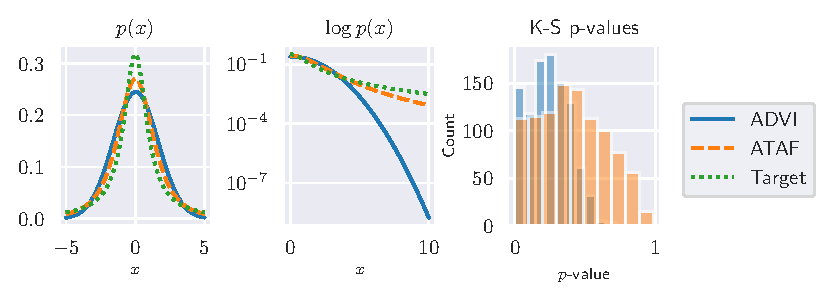
\includegraphics{../Figures/fat_tail_ks.pdf}
  \vspace{-6mm}
  \caption{
    When performing FTVI to approximate a $X \sim \text{Cauchy}(x_0 = 0, \gamma = 1)$ target (left panel, green dotted line),
    the use of a sub-Gaussian variational family (ADVI, solid blue line) can incur
    exponentially bad tail approximations (middle panel) compared to
    methods which permit heavier tails (ATAF, green dashed line) and results in
    samples which are more similar to the target (as measured by $1000$ repeats of
    1-sample $N=100$ Kolmogorov-Smirnov $p$-values, right panel).
    % \michael{Why does (b) look so good; are the tails really perfect, of if we went out to 15 or 30 on the X axis.  It might be good to show ATAF is much better but still not perfect.  Also, what is the X axis on each figure.  }
  }
  \label{fig:cauchy_normal_student}
\end{figure*}

\section{Normal-normal location mixture}
\label{sec:normal-normal-location-mixture}

We consider a Normal-Normal conjugate inference problem where the posterior
is known to be a Normal distribution as well. Here, we aim to show that ATAF
performs no worse than ADVI because $\text{StudentT}(\nu) \to N(0, 1)$ as $\nu \to \infty$.
\Cref{fig:normal_normal} shows the resulting density approximation, which can
be seen to be reasonable for both a Normal base distribution (the ``correct'' one)
and a StudentT base distribution. This suggests that mis-specification (i.e., heavier
tails in the base distribution than the target) may not be too problematic.

\begin{figure}
  \centering
  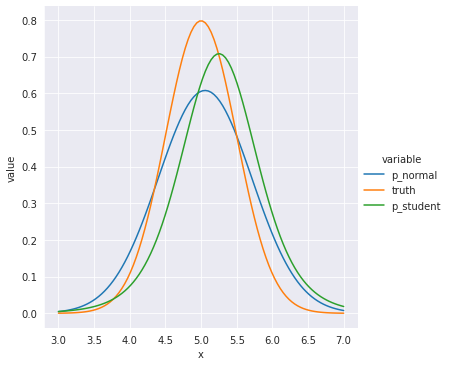
\includegraphics[width=0.6\textwidth]{../Figures/normal_normal_posterior.png}
  \caption{VI against a Normal posterior}
  \label{fig:normal_normal}
\end{figure}

\section{Example of non-existence of tail parameter due to oscillations}
\label{eg:spiral}

Consider $\text{StudentT}(\nu=1) \otimes \text{StudentT}(\nu=2)$ and ``spin'' it
using the radial transformation $(r,\theta) \mapsto (r,r+\theta)$ (\Cref{fig:spiral}). Due to
oscillations, $\alpha_X(v)$ is not well defined for all $v \in \cS^{1}$.


\begin{figure*}[htbp]
    \centering
    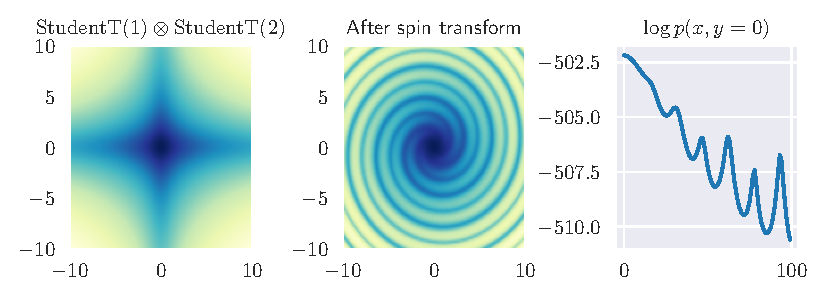
\includegraphics[scale=0.8]{Figures/spiral.pdf}
    % 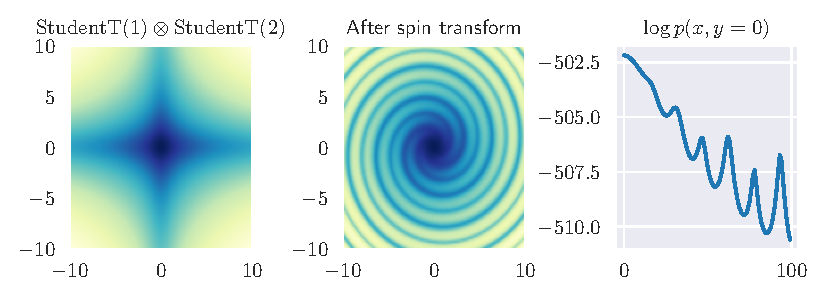
\includegraphics[trim={0 0 9cm 0},clip]{Figures/spiral.pdf}\\
    % 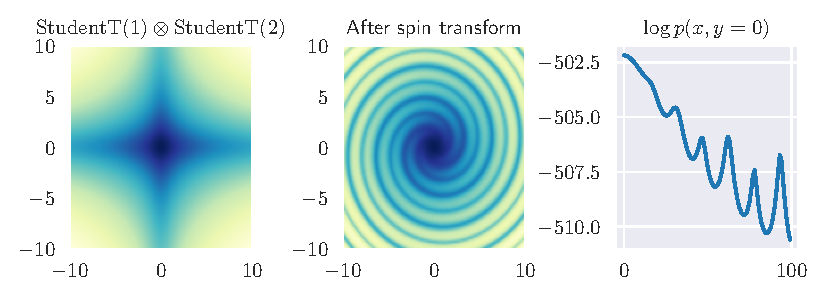
\includegraphics[trim={5cm 0 4.9cm 0},clip]{Figures/spiral.pdf}\\
    % 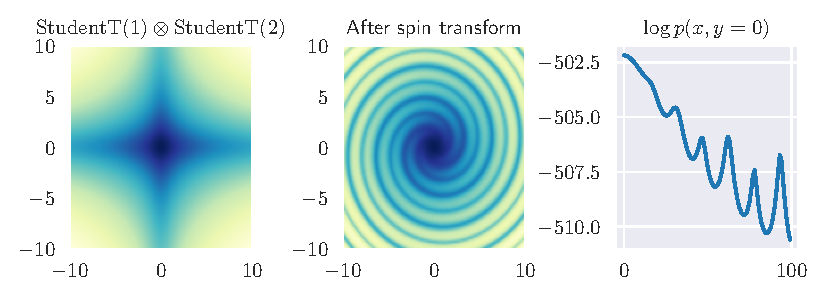
\includegraphics[trim={9.3cm 0 0cm 0},clip]{Figures/spiral.pdf}\\
    \caption{Taking a tail-anisotropic distribution (top) and ``spinning'' it (middle) results in
        one-dimensional projections which oscillate between tail parameters (as seen in
        $\log p(\braket{X,e_0})$ in bottom panel) and cause $\alpha_X(\cdot)$ to be not well defined.
    }
    \label{fig:spiral}
\end{figure*}

\section{Additional details for experiments}
\label{sec:additional-exp-details}

All experiments were performed on an Intel i8700K with 32GB RAM and a NVIDIA GTX 1080
running PyTorch 1.9.0 / Python 3.8.5 / CUDA 11.2 / Ubuntu Linux 20.04 via Windows Subsystem for Linux.
For all flow-transforms $\Phi_{\text{Flow}}$ we used inverse autoregressive flows \citep{kingma2016improved} with a
dense autoregressive conditioner consisting of two layers of either 32 or 256 hidden units depending on problem (see code for details) and
ELU activation functions.
As described in \cite{jaini2020tails}, TAF is trained by including $\nu$ within the Adam optimizer alongside other flow parameters. For ATAF, we include all $\nu_i$ within the optimizer.
Models were trained using the Adam optimizer with $10^{-3}$ learning rate
for 10000 iterations, which we found empirically in all our experiments to result in negligible change in ELBO
at the end of training.

For \cref{tab:diamonds} and \cref{tab:eight_schools}, the flow transform $\Phi_{\text{Flow}}$ used for ADVI, TAF, and ATAF
are comprised of two hidden layers of 32 units each. NUTS uses no such flow transform. Variational parameters for each normalizing flow were initialized
using \texttt{torch}'s default Kaiming initialization \citep{he2015delving} Additionally, the tail parameters $\nu_i$
used in ATAF were initialized to all be equal to the tail parameters learned from training TAF. We empirically observed
this resulted in more stable results (less variation in ELBO / $\log p(y)$ across trials), which may be due to
the absence of outliers when using a Gaussian base distribution resulting in more stable ELBO gradients. This suggests
other techniques for handling outliers such as winsorization may also be helpful, and we leave further investigation
for future work.


For \cref{fig:blr-anisotropic}, the closed-form posterior was computed over a finite element grid to produce
the ``Target'' row. A similar progressive training scheme used for \cref{tab:diamonds} was also used here, with
the TAF flow transform $\Phi_{\text{Flow}}$ was initialized from the result of ADVI and ATAF additionally initialized
all tail parameters $\nu_i$ based on the final shared tail parameter obtained from TAF training. Tails are computed
along the $\beta = 1$ or $\sigma = 1$ axes because the posterior is identically zero for $\sigma = 0$ hence it reveals
no information about the tails.

\bibliography{refs_ftvi}

\end{document}
